\documentclass[tikz,border=8pt]{standalone}

\usetikzlibrary{arrows.meta,matrix,fit}

\newlength{\NodeSize}
\newlength{\SiblingDistance}
\newlength{\LevelDistance}
\newlength{\LabelOffset}

\setlength{\NodeSize}{6mm}
\setlength{\SiblingDistance}{6mm}
\setlength{\LevelDistance}{10mm}

\tikzset{
  tree node/.style={draw, circle, minimum size=\NodeSize, inner sep=0pt},
}

\begin{document}

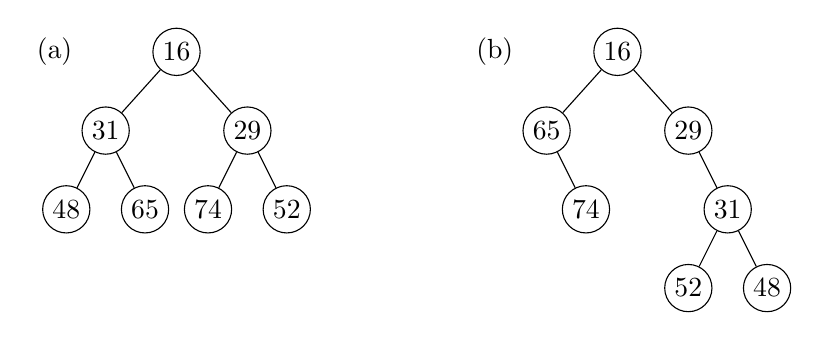
\begin{tikzpicture}[
    >=latex,
    level distance=\LevelDistance,
    level 1/.style={sibling distance=18mm},
    level 2/.style={sibling distance=10mm},
    level 3/.style={sibling distance=10mm}
  ]
  \begin{scope}[xshift=-28mm]
    \node[tree node] {16}
    child {
      node[tree node] {31}
      child {node[tree node] {48}}
      child {node[tree node] {65}}
    }
    child {
      node[tree node] {29}
      child {node[tree node] {74}}
      child {node[tree node] {52}}
    };

    \node[anchor=east] at (-12mm,0mm) {(a)};
  \end{scope}

  \begin{scope}[xshift=28mm]
    \node[tree node] {16}
    child {
      node[tree node] {65}
      child[missing]
      child {node[tree node] {74}}
    }
    child {
      node[tree node] {29}
      child[missing]
      child {
        node[tree node] {31}
        child {node[tree node] {52}}
        child {node[tree node] {48}}
      }
    };
    \node[anchor=east] at (-12mm,0mm) {(b)};
  \end{scope}

\end{tikzpicture}

\end{document}
